%\documentclass[unicode]{beamer}
\documentclass[unicode,hyperref={unicode=true}]{beamer}
\mode<presentation>
{
%  \useoutertheme{shadow}
%  \useinnertheme{rounded}
  \usecolortheme[RGB={55,109,160}]{structure}
%  \usetheme[height=7mm]{Rochester}
%  \usetheme{default}
%  \usetheme{Warsaw}
%  \usetheme{Frankfurt}
  \usetheme{Dresden}
%  \setbeamercolor{normal text}{bg=black,fg=white}
  \setbeamertemplate{navigation symbols}{}
  \setbeamertemplate{blocks}[rounded][shadow=true]
  \setbeamertemplate{items}[ball]
  \setbeamercovered{invisible}
}

\defbeamertemplate*{footline}{infolines theme}
{
  \leavevmode%
  \hbox{%
  \begin{beamercolorbox}[wd=\paperwidth,ht=2.25ex,dp=1ex,right]{date in head/foot}%
    \insertframenumber{} / \inserttotalframenumber\hspace*{2ex}
  \end{beamercolorbox}}%
  \vskip0pt%
}

% \setbeamertemplate{headline}{
%   \leavevmode
%  \hbox{%
%  \begin{beamercolorbox}[wd=\paperwidth,ht=3.25ex,dp=1ex,right]{date in head/foot}%
%    Институт системного программирования \\ Российская академия наук
%    \insertframenumber{} / \inserttotalframenumber\hspace*{2ex}
%  \end{beamercolorbox}}%
%  \vskip0pt%
%   \includegraphics[width=\textwidth]{logo-cmb.png}%
%}

\setbeamertemplate{headline}{
	\begin{beamercolorbox}[wd=\paperwidth,ht=3.25ex,dp=1ex,left]{date in head/foot}
		~~\insertsection
	\end{beamercolorbox}
}

\setbeamerfont{section title}{parent=title}
\setbeamercolor{section title}{parent=titlelike}
\defbeamertemplate*{section page kb}{default}[1][]
{
  \centering
	\begin{beamercolorbox}[sep=8pt,center,#1]{section title}
	  \usebeamerfont{section title}\insertsection\par
	\end{beamercolorbox}
}
\newcommand*{\sectionpagekb}{\usebeamertemplate*{section page kb}}
\setbeamercolor{block title}{use=structure,fg=white,bg=structure.fg!75!black}

\usepackage{etex}
\usepackage[T1]{fontenc}
\usepackage[utf8]{inputenc}
\usepackage[russian]{babel}
\usepackage{graphicx}
\usepackage{fancyvrb}
\usepackage{shortvrb}
\usepackage{amsthm}
\usepackage[]{url}
%\MakeShortVerb{!}
\usepackage{listings}
\usepackage{enumerate}
\usepackage{tikz}
\usepackage{pgf-pie}
\usepackage{xy}
\usepackage{algorithm}
\usepackage{algorithmicx}
\usepackage{algpseudocode}
\usepackage{latexsym}
\usepackage{subfig}
\usepackage{tikz}
\usepackage{dirtree}
\usetikzlibrary{positioning,arrows}
%\lstset{basicstyle=\ttfamily,language=lisp}

\theoremstyle{definition}
\newtheorem{mydef}{Определение}
\theoremstyle{plain}
\newtheorem{stmt}{Утверждение}
%\theoremstyle{plain}
%\newtheorem{lemma}{Лемма}

\title[]
{Автоматизация разработки моделей устройств и вычислительных машин для QEMU}

\author[]{Ефимов Василий}

\institute[]{ИСП РАН}

\date[]{число месяц  2017}

\begin{document}

\begin{frame}
\titlepage
\end{frame}



\begin{frame}{Проблема}
Разработка моделей устройств и вычислительных машин для QEMU~--- это трудоёмкий
процесс. В связи с повысившейся заинтересованностью в расширении QEMU новыми
вычислительными машинами требуется его ускорить. Ускорения предлагается достичь
за счёт автоматизации.
\end{frame}



\begin{frame}{Цели работы}
Целью работы является автоматизация процесса разработки моделей устройств и
вычислительных машин для эмулятора QEMU.

\vskip.5cm

{Для достижения поставленной цели были выполнены следующие задачи:}

\begin{itemize}
\item поиск в исследуемом процессе автоматизируемых этапов;
\item разработка и реализация методов автоматизации;
\item повышение удобства и эффективности реализованного инструмента.
\end{itemize}
\end{frame}



\section{Подход к автоматизации}
\frame{\sectionpagekb}



\begin{frame}{Процесс разработки}
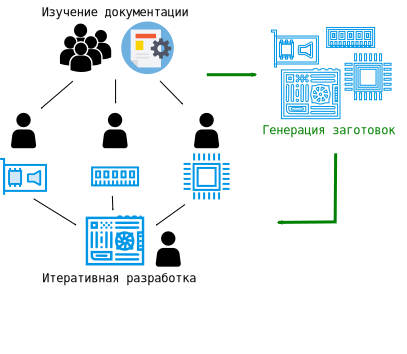
\includegraphics[width=\linewidth]{workflow.png}
\end{frame}



\begin{frame}{Устройство}

\begin{itemize}
\item Развитый обобщающий API
\item Много формального интерфейсного кода
\item Индивидуальный код сосредоточен в чётко определённых местах
\end{itemize}

\begin{center}
Можно по краткому перечню параметров сгенерировать сравнительно большую
заготовку.
\end{center}

\end{frame}



\begin{frame}{Вычислительная машина}

\begin{itemize}
\item Декларативный характер определения
\item Применяется объектная модель
\item Сложная система взаимосвязей, тяжело поддающаяся восприятию в форме
программного кода
\end{itemize}

\begin{center}
Можно разработать графический редактор, генерирующий {\it{}почти}
работоспособную модель.
\end{center}

\end{frame}



\section{Разработанный инструмент}
\frame{\sectionpagekb}


\begin{frame}{}
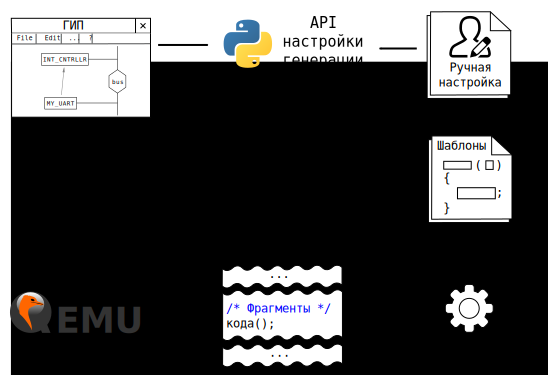
\includegraphics[width=\linewidth]{main.png}
\end{frame}



\begin{frame}{API настройки генерации устройства}
\begin{center}
\begin{tabular}{l|r}
Класс устройства & Настройки \\
\hline
Любой            & таймеры \\
                 & символьные и блочные устройства \\
                 & сетевой интерфейс \\
\hline
Устройство       & MMIO \\
системной        & PMIO \\
шины             & in/out IRQ \\
\hline
Функция          & BAR \\
PCI(E)           & out IRQ (INTx) \\
устройства       & MSI(X) \\
                 & идентификационная информация
\end{tabular}
\end{center}
\end{frame}



\begin{frame}{ГИ настройки генерации устройства}
\begin{center}
PCI Fast Ethernet контроллер из С2600
\end{center}
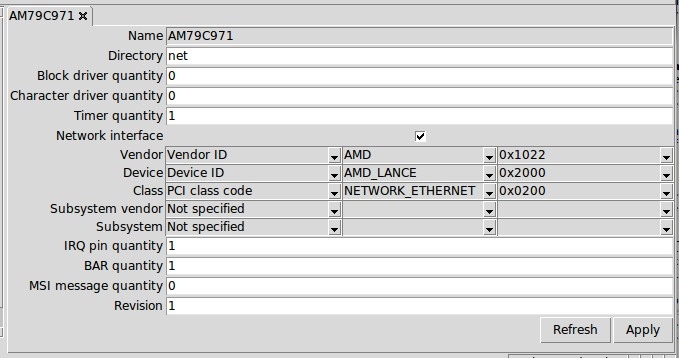
\includegraphics[width=\linewidth]{AM79C971.jpg}
\end{frame}



\begin{frame}[fragile]{Код настройки генерации устройства}

\lstset{language=Python}
\begin{lstlisting}
obj43 = SysBusDeviceDescription(
    name = "CISCO remote",
    directory = "char",
    out_irq_num = 0,
    in_irq_num = 0,
    mmio_num = 0x1,
    pio_num = 0,
    nic_num = 0,
    timer_num = 0,
    char_num = 0x1,
    block_num = 0x1
)
\end{lstlisting}

\end{frame}



\begin{frame}[fragile]{API компоновки вычислительной машины}

\dirtree{%
.1 Node .
    .2 BusNode .
        .3 SystemBusNode .
        .3 PCIExpressBusNode .
        .3 [ISA, IDE, I2C]BusNode .
    .2 DeviceNode .
        .3 SystemBusDeviceNode .
        .3 PCIExpressDeviceNode .
    .2 IRQLine .
    .2 IRQHub .
    .2 MemoryNode .
        .3 MemoryLeafNode .
            .4 MemoryAliasNode .
            .4 MemoryRAMNode .
            .4 MemoryROMNode .
}
\end{frame}



\begin{frame}{Схема вычислительной машины}
\begin{center}
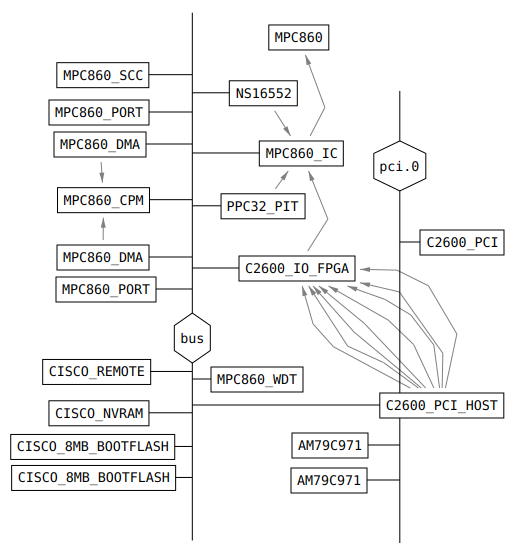
\includegraphics[height=0.9\textheight]{C2600.png}
\end{center}
\end{frame}



\begin{frame}{ГИ настройки интеграции устройства}
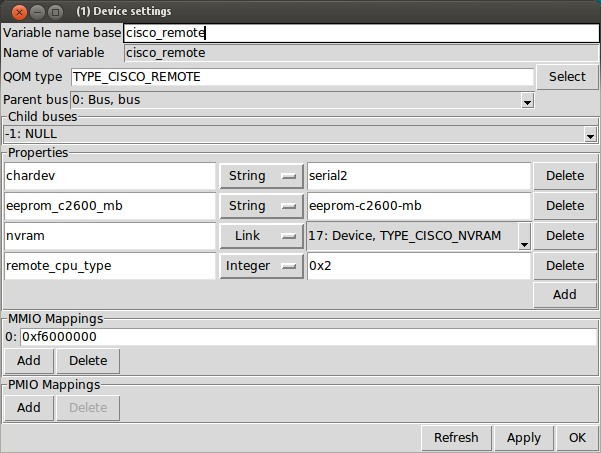
\includegraphics[height=0.9\textheight]{REMOTE.jpg}
\end{frame}



\begin{frame}[fragile]{Код настройки интеграции устройства}

\lstset{language=Python}
\begin{lstlisting}
obj3 = SystemBusDeviceNode(
    qom_type = "TYPE_CISCO_REMOTE",
    system_bus = obj1,
    mmio = [ 0xf6000000 ]
)
obj3.properties.extend([
    QOMPropertyValue(QOMPropertyTypeString,
        "chardev", "serial2"),
    QOMPropertyValue(QOMPropertyTypeString,
        "eeprom_c2600_mb", "eeprom-c2600-mb"),
    QOMPropertyValue(QOMPropertyTypeLink,
        "nvram", obj2),
    QOMPropertyValue(QOMPropertyTypeInteger,
        "remote_cpu_type", 0x2)
])
\end{lstlisting}

\end{frame}



\begin{frame}{Устройство генератора}

\includegraphics[height=0.9\textheight]{generation.png}
\end{frame}



\begin{frame}{Модель языка программирования}
\end{frame}



\begin{frame}{Модель файла с исходным кодом}
\end{frame}



\begin{frame}{Анализ QEMU, взаимосвязь}
\end{frame}



\section{Примеры}
\frame{\sectionpagekb}



\begin{frame}{С2600 (C2621XM)}
Описание
\end{frame}



\begin{frame}{}
Схема
\end{frame}



\begin{frame}{}
Статистика
\end{frame}



\begin{frame}{Intel Q35}
Описание
\end{frame}



\begin{frame}{}
Схема
\end{frame}



\begin{frame}{}
Статистика
\end{frame}



\begin{frame}{Слайд с таблицей}
\begin{itemize}
\item ...,
\end{itemize}

\begin{center}
{\Large\color{structure.fg} Результаты} \\
\begin{tabular}{|r|c|c|c|}
\hline
Тест & без & с & \% \\
 & оптимизаций & оптимизациями & \\
\hline
a & 1 & 2 & \color{green!40!black}{3} \\
b & 4 & 5 & 63 \\
c & 237 & 123485 & 0.1 \\
d & 237 & 2241 & \color{green!40!black}{3} \\
e & 15 & 15 & \color{green!40!black}{1} \\
\hline
\end{tabular}
\end{center}

\end{frame}

\begin{frame}{Слайд с диаграммами}
\vskip8pt
\begin{tabular}{cc}
До изменений & После изменений \\
\resizebox{0.46\linewidth}{!}{
\begin{tikzpicture}
\pie{4.42/нехватка, 37.31/конец ББ, 58.27/вызовы}
\end{tikzpicture}} &
\resizebox{0.46\linewidth}{!}{
\begin{tikzpicture}
\pie{0.51/нехватка, 38.69/конец ББ, 60.80/вызовы}
\end{tikzpicture}}
\end{tabular}
\end{frame}



\begin{frame}{Слайд с нумерацией}
\begin{enumerate}
\item\label{strat_all} пункт
\item\label{strat_sync} ...
\item\label{strat_none} ...
\end{enumerate}

\vskip.5cm

Отступ
\end{frame}

\begin{frame}{Слайд с определениями}
\begin{mydef}
Определение 1
\end{mydef}
\begin{mydef}
Определение 1
\end{mydef}
\end{frame}

\begin{frame}{Слайд с графом}
\begin{center}
\resizebox{!}{0.85\textheight}{%
\begin{tikzpicture}[scale = 0.6]
	\draw[very thick] (3,20) rectangle (7,25);
	\draw[very thick] (3,23.5) -- (7, 23.5);
	\node at (5,24.15){BB4};
	\node at (5,22.75){var};

	\draw[very thick] (0,0) rectangle (4,5);
	\draw[very thick] (0,3.5) -- (4, 3.5);
	\node at (2,4.15){BB2};
	\node at (2,2.75){var};

	\draw[very thick] (0,10) rectangle (4,15);
	\draw[very thick] (0,13.5) -- (4, 13.5);
	\node at (2,14.15){BB0};
	\node at (2,12.75){var};

	\draw[very thick] (6,0) rectangle (10,5);
	\draw[very thick] (6,3.5) -- (10, 3.5);
	\node at (8,4.15){BB3};
	\node at (8,2.75){var};

	\draw[very thick] (6,10) rectangle (10,15);
	\draw[very thick] (6,13.5) -- (10, 13.5);
	\node at (8,14.15){BB1};
	\node at (8,12.75){var};

	\draw[very thick,->,>=stealth',purple] (2,10) -- (2,5);
	\draw[very thick,->,>=stealth',purple] (8,10) -- (2,5);
	\draw[very thick,->,>=stealth',purple] (8,10) -- (8,5);
	\draw[very thick,->,>=stealth',blue] (5,20) -- (2,15);
	\draw[very thick,->,>=stealth',blue] (5,20) -- (8,15);
\end{tikzpicture}
}
\end{center}
\end{frame}

\begin{frame}{}
\begin{block}{Слайд с алгоритмом}
\begin{algorithmic}
\Procedure{Combined-Reg-Alloc}{$TB$}
	\ForAll{$b\in B(TB)$}\Comment{Начальная инициализация}
		\State $b^{pre}\gets \varnothing$
		\State $b^{post}\gets \varnothing$
	\EndFor
	\ForAll{$J\in \mathbb{J}(TB)$}\Comment{Основной цикл}
		\State $regmap\gets$ \textsc{Compute-Register-Mapping}($J$)
		\ForAll{$(src, dst)\in J$}
			\State $src^{post}\gets regmap$
			\State $dst^{pre}\gets regmap$
		\EndFor
	\EndFor
	\ForAll{$b\in B(TB)$}
		\State \textsc{Local-Reg-Alloc}($b$)
	\EndFor
\EndProcedure
\end{algorithmic}
\end{block}
\end{frame}

\begin{frame}{Текущее состояние}
\end{frame}

\begin{frame}{Экспериментальные результаты}
\center
\end{frame}

\section{Результаты}
\frame{\sectionpagekb}

\begin{frame}{Результаты}
\end{frame}

\end{document}
